\documentclass{article}
% For math environments
\usepackage{amsmath, amsfonts}
% For links
\usepackage[hidelinks]{hyperref}
% So space it put between paragraphs
\usepackage{parskip}
% For figures
\usepackage{tikz}
% Set the margins to not be ridiculous
\usepackage[margin=0.75in]{geometry}
% For multiple columns
\usepackage{multicol}
% For controlling enum/itemize spacing and indentation
\usepackage{enumitem}

% For tikz plots
\usepackage{pgfplots}
% This isn't needed but avoids a compiler warning
\pgfplotsset{compat=1.16}

% Allow multi-line equations to be broken across pages
\allowdisplaybreaks

% Use @ as a letter
\makeatletter

% Scale down all tikz coordinates while maintaining font size
\tikzset{every picture/.style={scale=0.45, every picture/.style={}}}


% Macros
% Monospace code
\def\code#1{\texttt{#1}}

% Greek letters
\def\a{\alpha}
\def\b{\beta}
\def\g{\gamma}
\def\d{\delta}
\def\D{\Delta}

% Some common sets
\def\es{\varnothing}
\def\ints{{\mathbb{Z}}}

% Commands that make life easier
\newcommand\gath[1]{\begin{gather} #1 \end{gather}}
\newcommand\gaths[1]{\begin{gather*} #1 \end{gather*}}
\newcommand\ali[1]{\begin{align} #1 \end{align}}
\newcommand\parens[1]{\left( #1 \right)}
\newcommand\squares[1]{\left[ #1 \right]}
\newcommand\braces[1]{\left\{ #1 \right\}}
\newcommand\angles[1]{\left\langle #1 \right\rangle}
\newcommand\deriv[2]{\frac{d #1}{d #2}}
\newcommand\abs[1]{\left| #1 \right|}
\newcommand\floor[1]{\left\lfloor #1 \right\rfloor}
\newcommand\ceil[1]{\left\lceil #1 \right\rceil}
\DeclareMathOperator{\lcm}{lcm}
\def\non{\nonumber \\}
\newcommand\unit[1]{~\mathrm{#1}}
\newcommand\combos[2]{{}_{#1}C_{#2}}

% Set stuff
\def\ss{\subseteq}

% Multiline equation space
\def\mlesp{\hspace{1.2cm}}

% For grid diagrams
\newcommand\gridbox[3]{\draw (#1,#2) rectangle (#1+1,#2+1) node[pos=.5] {#3};}
\newcommand\gridboxh[3]{\draw[fill=red!20] (#1,#2) rectangle (#1+1,#2+1) node[pos=.5] {#3};}
\newcommand\gridboxb[3]{\draw[fill=black] (#1,#2) rectangle (#1+1,#2+1) node[pos=.5] {#3};}
\newcommand\gridsym[3]{\node at (#1+0.5,#2+0.5) {$#3$};}
\newcommand\gridblank[2]{\filldraw[draw=gray, color=gray] (#1,#2) rectangle (#1+1,#2+1);}
\newcommand\gridcirc[2]{\draw (#1 + 0.5,#2 + 0.5) circle (0.25);}
\newcommand\cwlab[3]{
  \def\dd{0.15}
  \draw (#1 + \dd - 0.03, #2 + 1 - \dd) node {\scriptsize #3};
}

\def\bbw{3.5}
\def\bbh{2}
\newcommand\bigbox[3]{\draw (#1*\bbw,#2*\bbh) rectangle (#1*\bbw+\bbw,#2*\bbh+\bbh) node[pos=.5] {#3};}
\newcommand\bbtextr[3]{\node[right] at (#1*\bbw,#2*\bbh+0.5*\bbh) {#3};}
\newcommand\bbtextb[3]{\node[align=center] at (#1*\bbw+0.5*\bbw,#2*\bbh+0.5*\bbh) {#3};}

% Box puzzle stock answer
\newcommand\boxans[1]{
  Logic was used to deduce the solution:

  #1

  This was verified using Python as well as shown to be unique with a brute force approach.
}

% Standard crossnumber grid
\newcommand\crossnumstd[9]{
  \begin{center}
    \begin{tikzpicture}[scale=2]
      \gridbox{0}{2}{#1}
      \gridbox{1}{2}{#2}
      \gridbox{2}{2}{#3}
      \gridbox{0}{1}{#4}
      \gridbox{1}{1}{#5}
      \gridbox{2}{1}{#6}
      \gridbox{0}{0}{#7}
      \gridbox{1}{0}{#8}
      \gridbox{2}{0}{#9}

      % Labels
      \cwlab{0}{2}{1}
      \cwlab{1}{2}{2}
      \cwlab{2}{2}{3}
      \cwlab{0}{1}{4}
      \cwlab{0}{0}{5}
    \end{tikzpicture}
  \end{center}
}

% Multiple numbers
\newcommand\mn[1]{$#1$'s}

% Commands for problems
\newcommand\problem[4]{
\section*{#1}

\textbf{Question:} #3

\textbf{Answer:} #2

\textbf{Explanation:} #4
}
\newcommand\aproblem[4]{\problem{Dec #1}{#2}{#3}{#4}}
\newcommand\cproblem[4]{\problem{Problem #1}{#2}{#3}{#4}}

\newcommand\xref@advent[2]{#1 Advent, Dec~#2 problem}
\newcommand\xref@card[2]{#1 Christmas Card, Problem #2}

% For answered verified with Python
\newcommand{\verified}{This was verified with a brute-force Python program.}

\def\advent@xxi@i{
  The geometric mean of a set of $n$ numbers can be computed by multiplying together all the numbers then computing the $n$th root of the result.

  The factors of $4$ are $1$, $2$ and $4$. The geometric mean of these is 2.

  The factors of $6$ are $1$, $2$, $3$, and $6$. The geometric mean of these is $\sqrt{6}$.

  The geometric mean of all the factors of today's number is $22$.
}

\def\advent@xxi@ii{
  The number $7n$ has $37$ factors (including $1$ and the number itself).
  How many factors does $8n$ have?
}

\def\advent@xxi@iii{
  If you write out the numbers from $1$ to $1000$ (inclusive), how many times will you write the digit $0$?
}

\def\advent@xxi@iv{
  Put the digits $1$ to $9$ (using each digit exactly once) in the boxes so that the sums are correct.
  The sums should be read left to right and top to bottom ignoring the usual order of operations.
  For example, $4 + 3 \times 2$ is $14$, not $10$.
  Today's number is the product of the numbers in the red boxes.

  \grid@advent@xxi@iv{}{}{}{}{}{}{}{}{}
}

\def\advent@xxi@v{
  How many different isosceles triangles are there whose perimeter is $50$ units, and whose area is an integer number of units squared?

  (Two triangles that are rotations, reflections and translations of each other are counted as the same triangle. Triangles with an area of 0 should not be counted.)
}

\def\advent@xxi@vi{
  When $12345$ is divided by today's number, the remainder is $205$.
  When $6789$ is divided by today's number, the remainder is $112$.
}

\newcommand\dec@ai{0.30901699437494745}
\newcommand\dec@aii{0.8090169943749475}
\newcommand\dec@bi{0.5877852522924731}
\newcommand\dec@bii{0.9510565162951535}
\newcommand\decagon[5]{
  \def\ai{\dec@ai*#3+#1}
  \def\aii{\dec@aii*#3+#1}
  \def\bi{\dec@bi*#3+#2}
  \def\bii{\dec@bii*#3+#2}
  \draw (#3+#1, #2) -- (\aii, \bi) -- (\ai, \bii) -- (-\ai, \bii) -- (-\aii, \bi) -- (-#3+#1, #2) -- (-\aii, -\bi) -- (-\ai, -\bii) -- (\ai, -\bii) -- (\aii, -\bi) -- cycle;
  \fill[fill=red] (-\ai, -\bii) -- (#4*#3+#1, #5*#3+#2) -- (\ai, -\bii) -- cycle;
}
\def\advent@xxi@vii{
  The picture below shows eight regular decagons.
  In each decagon, a red triangle has been drawn with vertices at three of the vertices of the decagon.

  \begin{center}
    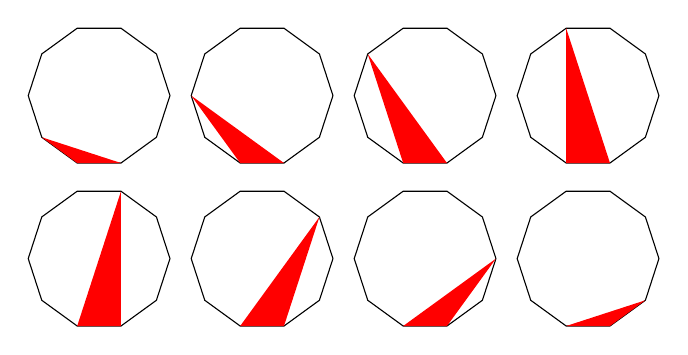
\begin{tikzpicture}
      \def\dr{2}
      \def\spc{2.3*\dr}

      \decagon{0*\spc}{\spc}{\dr}{-\dec@aii}{-\dec@bi}
      \decagon{1*\spc}{\spc}{\dr}{-1}{0}
      \decagon{2*\spc}{\spc}{\dr}{-\dec@aii}{\dec@bi}
      \decagon{3*\spc}{\spc}{\dr}{-\dec@ai}{\dec@bii}

      \decagon{0*\spc}{0}{\dr}{\dec@ai}{\dec@bii}
      \decagon{1*\spc}{0}{\dr}{\dec@aii}{\dec@bi}
      \decagon{2*\spc}{0}{\dr}{1}{0}
      \decagon{3*\spc}{0}{\dr}{\dec@aii}{-\dec@bi}
    \end{tikzpicture}
  \end{center}

  The area of each decagon is $240$.
  What is the total area of all the red triangles?
}

\def\advent@xxi@viii{
  The sum of three integers is $51$.
  The product of the same three integers is $836$. What is the product of largest integer and the second-largest integer?
}

\def\advent@xxi@ix{
  Eve writes down a sequence of consecutive positive integers (she writes more than one number).
  The sum of the numbers Eve has written down is $844$.
  Today's number is the smallest integer that Eve has written down.
}

\def\advent@xxi@x{
  Put the digits $1$ to $9$ (using each digit exactly once) in the boxes so that the sums are correct.
  Today's number is the largest number you can make using the digits in the red boxes.

  \grid@advent@xxi@x{}{}{}{}{}{}{}{}{}
}

\def\advent@xxi@xi{
  The integers are written in a triangle as shown below:
  \begin{center}
    \begin{tabular}{ccccccc}
         &    &    & 1    &    &    &    \\
         &    & 2  & 3    & 4  &    &    \\
         & 5  & 6  & 7    & 8  & 9  &    \\
      10 & 11 & 12 & 13   & 14 & 15 & 16 \\
         &    &    & etc. &    &    &
    \end{tabular}
  \end{center}
  Today's number appears directly above the number $750$ in the triangle of integers.
}

\def\advent@xxi@abgrid{
  \begin{center}
    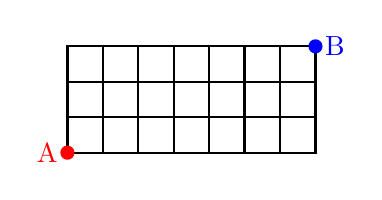
\begin{tikzpicture}
      \def\gs{1}
      % Grid
      \foreach \i in {0,...,6}{
          \foreach \j in {0,...,2}{
              \draw[thick] (\i * \gs, \j * \gs) rectangle (\i * \gs + \gs, \j * \gs + \gs);
            }
        }
      % Points
      \fill[color=red] (0, 0) circle (0.2) node[color=red,left] {A};
      \fill[color=blue] (7*\gs, 3*\gs) circle (0.2) node[color=blue,right] {B};
    \end{tikzpicture}
  \end{center}
}
\def\advent@xxi@xii{
  You start at the point marked A in the picture below. You want to get to the point marked B.
  You may travel \textbf{to the right} or \textbf{upwards} along the black lines.

  \advent@xxi@abgrid

  Today's number is the total number of possible routes to get from A to B.
}

\def\advent@xxi@xiii{
  The diagram below shows three circles and two triangles.
  The three circles all meet at one point.
  The vertices of the smaller red triangle are at the centers of the circles.
  The lines connecting the vertices of the larger blue triangle to the point where all three circles meet are diameters of the three circles.

  \begin{center}
    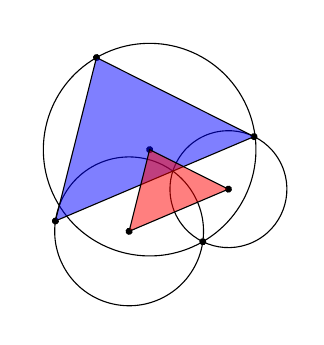
\begin{tikzpicture}[rotate=30,transform shape]
      \def\bcr{3}
      \def\scr{0.55*\bcr}
      \def\sca{34}
      \def\mcr{0.7*\bcr}
      \def\mca{142}
      \def\pr{0.1}

      % Circles
      \draw (0, \bcr) circle (\bcr);
      \draw (\sca: \scr) circle (\scr);
      \draw (\mca: \mcr) circle (\mcr);

      % Points
      \fill (0, 0) circle (\pr);
      \fill (0, \bcr) circle (\pr);
      \fill (0, 2*\bcr) circle (\pr);
      \fill (\sca: \scr) circle (\pr);
      \fill (\sca: 2*\scr) circle (\pr);
      \fill (\mca: \mcr) circle (\pr);
      \fill (\mca: 2*\mcr) circle (\pr);

      % Triangles
      \draw[fill=blue,fill opacity=0.5] (\mca: 2*\mcr) -- (0, 2*\bcr) -- (\sca: 2*\scr) -- cycle;
      \draw[fill=red,fill opacity=0.5] (\mca: \mcr) -- (0, \bcr) -- (\sca: \scr) -- cycle;
    \end{tikzpicture}
  \end{center}

  The area of the smaller red triangle is $226$.
  What is the area of the larger blue triangle?
}

\def\advent@xxi@xiv{
  You start at the point marked A in the picture below.
  You want to get to the point marked B.
  You may travel \textbf{to the right}, \textbf{upwards}, or \textbf{to the left} along the black lines, but you cannot pass along the same line segment more than once.

  \advent@xxi@abgrid

  Today's number is the total number of possible routes to get from A to B.
}

\newcommand\pyramid@advent@xxi@xvi[6]{
  \begin{center}
    \begin{tabular}{cccccc}
      (row 1) &    &    & #1   &    &    \\
      (row 2) &    & #2 &      & #3 &    \\
      (row 3) & #4 &    & #5   &    & #6 \\
              &    &    & etc. &    &
    \end{tabular}
  \end{center}
}
\def\advent@xxi@xv{
  The odd numbers are written in a pyramid.

  \pyramid@advent@xxi@xvi{1}{3}{5}{7}{9}{11}

  What is the mean of the numbers in the 19th row?
}

\newcommand\grid@advent@xxi@xvi[9]{
  \begin{center}
    \begin{tikzpicture}[scale=2]
      \gridbox{0}{2}{#1}
      \gridbox{1}{2}{#2}
      \gridbox{2}{2}{#3}
      \gridbox{0}{1}{#4}
      \gridbox{1}{1}{#5}
      \gridbox{2}{1}{#6}
      \gridbox{0}{0}{#7}
      \gridbox{1}{0}{#8}
      \gridbox{2}{0}{#9}

      % Labels
      \cwlab{0}{2}{1}
      \cwlab{1}{2}{2}
      \cwlab{2}{2}{3}
      \cwlab{0}{1}{4}
      \cwlab{0}{0}{5}
    \end{tikzpicture}
  \end{center}
}
\def\advent@xxi@xvi{
  Each clue in this crossnumber is formed of two parts connected by a logical connective: AND means that both parts are true; NAND means that at most one part is true; OR means that at least one part is true; NOR means that neither part is true; XOR means that exactly one part is true; XNOR means that either both parts are false or both parts are true.
  No number starts with $0$.

  \begin{multicols}{2}
    \grid@advent@xxi@xvi{}{}{}{}{}{}{}{}{}

    \columnbreak

    \begin{enumerate}
      \item \textbf{1A} is a palindrome XNOR \textbf{1D} is a palindrome.
      \item \textbf{1A} is greater than $350$ NOR \textbf{1D} is less than $150$.
      \item \textbf{3D} is odd NAND \textbf{4A} and \textbf{2D} are equal.
      \item \textbf{3D} is prime XOR \textbf{5A} is odd.
      \item \textbf{4A} is a cube AND \textbf{2D} is a cube.
      \item The sum of the digits of \textbf{3D} is $2$ OR the sum of the digits of \textbf{5A} is $5$.
      \item Today's number is \textbf{1D}.
    \end{enumerate}
  \end{multicols}
}

\def\advent@xxi@xvii{
  The digital product of a number is computed by multiplying together all of its digits. For example, the digital product of $6273$ is $252$.

  Today's number is the smallest number whose digital product is $252$.
}

\def\advent@xxi@xviii{
  Put the digits $1$ to $9$ (using each digit exactly once) in the boxes so that the sums are correct.
  The sums should be read left to right and top to bottom ignoring the usual order of operations.
  For example, $4 + 3 \times 2$ is $14$, not $10$.
  Today's number is the product of the numbers in the red boxes.

  \grid@advent@xxi@xviii{}{}{}{}{}{}{}{}{}
}

\def\advent@xxi@xix{
  The equation $352x^3 - 528x^2 + 90 = 0$ has three distinct real-valued solutions.

  Today's number is the number of integers $a$ such that the equation $352x^3 - 528x^2 + a = 0$ has three distinct real-valued solutions.
}

\def\advent@xxi@xx{
  What is the area of the largest area triangle that has one side of length $32$ and one side of length $19$?
}

\newcommand\grid@advent@xxi@xxi[9]{
  \begin{center}
    \begin{tikzpicture}
      \bigbox{0}{3}{#1}
      \bigbox{1}{3}{#2}
      \bigbox{2}{3}{#3}
      \bbtextr{3}{3}{\textbf{today's number}}

      \bigbox{0}{2}{#4}
      \bigbox{1}{2}{#5}
      \bigbox{2}{2}{#6}
      \bbtextr{3}{2}{prime}

      \bigbox{0}{1}{#7}
      \bigbox{1}{1}{#8}
      \bigbox{2}{1}{#9}
      \bbtextr{3}{1}{square}

      \bbtextb{0}{0}{cube}
      \bbtextb{1}{0}{odd}
      \bbtextb{2}{0}{multiple\\of $11$}
    \end{tikzpicture}
  \end{center}
}
\def\advent@xxi@xxi{
  Arrange the digits $1$–$9$ (using each digit exactly once) so that the three digit number in: the middle row is a prime number; the bottom row is a square number; the left column is a cube number; the middle column is an odd number; the right column is a multiple of $11$.
  The $3$-digit number in the first row is today's number.

  \grid@advent@xxi@xxi{}{}{}{}{}{}{}{}{}
}

\def\advent@xxi@xxii{
  There are $12$ ways of placing $2$ tokens on a $2 \times 4$ grid so that no two tokens are next to each other horizontally, vertically or diagonally:

  \begin{center}
    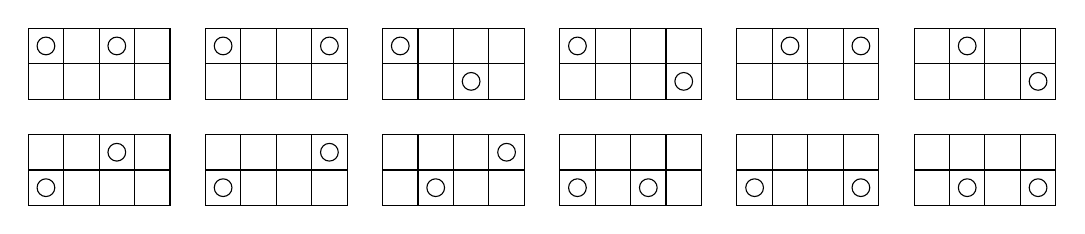
\begin{tikzpicture}
      % Draw all the grids
      \foreach \gi in {0,1}{
          \foreach \gj in {0,...,5}{
              \foreach \i in {0,1}{
                  \foreach \j in {0,...,3}{
                      \gridbox{5*\gj + \j}{3*\gi + \i}{}
                    }
                }
            }
        }

      % Place token circles
      \gridcirc{0}{4}
      \gridcirc{2}{4}
      \gridcirc{5}{4}
      \gridcirc{8}{4}
      \gridcirc{10}{4}
      \gridcirc{12}{3}
      \gridcirc{15}{4}
      \gridcirc{18}{3}
      \gridcirc{21}{4}
      \gridcirc{23}{4}
      \gridcirc{26}{4}
      \gridcirc{28}{3}
      \gridcirc{0}{0}
      \gridcirc{2}{1}
      \gridcirc{5}{0}
      \gridcirc{8}{1}
      \gridcirc{11}{0}
      \gridcirc{13}{1}
      \gridcirc{15}{0}
      \gridcirc{17}{0}
      \gridcirc{20}{0}
      \gridcirc{23}{0}
      \gridcirc{26}{0}
      \gridcirc{28}{0}
    \end{tikzpicture}
  \end{center}

  Today's number is the number of ways of placing $2$ tokens on a $2 \times 21$ grid so that no two tokens are next to each other horizontally, vertically or diagonally.
}

\def\advent@xxi@xxiii{
  I draw the parabola $y = x^2$ and mark points on the parabola at $x = 17$ and $x = -6$.
  I then draw a straight line connecting these two points.

  At which value of $y$ does this line intercept the $y$-axis?
}

\def\advent@xxi@xxiv{
  The digital product of a number is computed by multiplying together all of its digits.
  For example, the digital product of $1522$ is $20$.

  How many $12$-digit numbers are there whose digital product is $20$?
}

\def\card@xxi@i{
  What is the sum of all the odd integers between $0$ and $30$?
}

\def\card@xxi@ii{
  What is the sum of all the odd integers between $0$ and $5668$?
}

\def\card@xxi@iii{
  What is the smallest integer with a digital sum of $28$ and a digital product of $10000$?
}

\def\card@xxi@iv{
  What is the smallest integer with a digital sum of $41$ and a digital product of $432000$?
}

\def\card@xxi@v{
  What is the area of the largest area dodecagon that will fit inside a circle with area $111185 \pi$?
}

\def\card@xxi@vi{
  What is the area of the largest area heptagon that will fit inside a semicircle with area $115185 \pi$?
}

\def\card@xxi@vii{
  How many terms are there in the (simplified) expansion of $(x + y + z)^2$?
}

\def\card@xxi@viii{
  How many terms are there in the (simplified) expansion of $(x + y + z)^{41172}$?
}

\def\card@xxi@ix{
  What is the largest integer that cannot be written as $4a + 5b$ for non-negative integers $a$ and $b$?
}

\def\card@xxi@x{
  What is the largest integer that cannot be written as $83409a + 66608b$ for non-negative integers $a$ and $b$?
}

\def\card@xxi@xi{
  How many positive integers are there below $100$ whose digits are all non-zero and different?
}

\def\card@xxi@xii{
  How many positive integers are there whose digits are all non-zero and different?
}

\def\card@xxi@xiii{
  What is the only integer for which taking the geometric mean of all its factors (including $1$ and the number itself) gives $2$?
}

\def\card@xxi@xiv{
  What is the only integer for which taking the geometric mean of all its factors (including $1$ and the number itself) gives $25$?
}


\begin{document}

\title{MS Scroggs 2021 Christmas Card Solutions}
\author{Dan Whitman}
\date{}

\maketitle

Link to the online card: \href{https://www.mscroggs.co.uk/blog/92}{https://www.mscroggs.co.uk/blog/92}

\newcommand\Nodd[1]{N_\mathrm{o}\parens{#1}}

\cproblem{1}{225}{\card@xxi@i}{
  Let $\Nodd{n}$ denote the number of odd integers from $0$ to $n$ inclusive.
  Then clearly
  \ali{
    \Nodd{2n+1} &= \sum_{k=0}n (2k+1) = 2 \sum_{k=0}^n k + \sum_{k=0}^n 1 = 2 \sum_{k=1}^n k + (n+1) \non
    &= 2 \frac{n(n+1)}{2} + n + 1 = n(n+1) + n + 1 = n^2 + 2n + 1 \non
    &= (n+1)^2 \,. \label{eqn:01:Nodd}
  }
  In our case we have $\Nodd{30} = \Nodd{29}$ and $29 = 2 \cdot 14 + 1$ so that our answer is $\Nodd{30} = (14+1)^2 = 225$.
  This was verified in Python with brute force.
}

\cproblem{2}{8031556}{\card@xxi@ii}{
  From the previous problem, $\Nodd{5668} = \Nodd{5667}$ and $5667 = 2 \cdot 2833 + 1$, so that $\Nodd{5668} = (2833+1)^2 = 8031556$ by \eqref{eqn:01:Nodd} above.
  This was also verified in Python with brute force.
}

\def\pval{10000}
\cproblem{3}{445555}{\card@xxi@iii}{
  First, the prime factorization of $\pval$ is
  \gath{
    \pval = 2^4 5^4 \,.
  }
  The only digits that can be formed from products of these primes are $2$, $4 = 2^2$, $5$, and $8 = 2^3$, noting that, in particular, $2 \cdot 5 = 10$ is not a digit or is, for example $5^2 = 25$.
  Hence the answer must have four \mn{5} in it because these cannot be combined to create any other digits.
  The card board provides a hint here as it tells us that the answer has six digits.
  Since there must be four \mn{5}, the $2^4$ factor must comprise two digits.
  The only way to do this is with two \mn{4} since $4 \cdot 4 = 2^4$.
  Therefore the digits must be two $4$'s and four \mn{5}.
  Clearly the smallest number using these is found by just sorting the digits in ascending order, which is $445555$.
  This was verified with Python using brute force.
}

\def\pval{432000}
\cproblem{4}{44555666}{\card@xxi@iv}{
  Similar to the approach of the previous problem, the prime factorization of $\pval$ is
  \gath{
    \pval = 2^7 3^3 5^3 \,.
  }
  Here the only digits that can be formed from these prime factors are clearly $2$, $3$, $4 = 2^2$, $5$, $6=2 \cdot 3$, $8 = 2^3$, and $9 = 3^2$.
  Once again, the answer must contain three \mn{5} since these cannot be combined into other digits.
  Using the card board, the answer must have eight digits.
  So let the following denote the number of each digit in the answer:
  \begin{center}
    \begin{tabular}{c|c}
      Let & Digit \\
      \hline
      $a$ & 9     \\
      $b$ & 8     \\
      $c$ & 6     \\
      $d$ & 4     \\
      $e$ & 3     \\
      $f$ & 2
    \end{tabular}
  \end{center}
  Then, since three of the digits must be \mn{5}, we have
  \gath{
    a + b + c + d + e + f = 8 - 3 = 5 \,. \label{eqn:04:nd}
  }
  of the other digits.
  The digital sum then becomes
  \gath{
    9a + 8b + 5 \cdot 3 + 6c + 4d + 3e + 2f = 41 \non
    9a + 8b + 6c + 4d + 3e + 2f = 26 \label{eqn:04:ds}
  }
  Since \mn{9} use two \mn{3}, \mn{6} use one $3$, and we must have three $3$'s to achieve the digital product, it has to be that
  \gath{
    2a + c + e = 3 \non
    e = 3 - 2a - c \label{eqn:04:3s}
  }
  Similarly, for the digits that use \mn{2}, we must have
  \gath{
    3b + c + 2d + f = 7 \non
    f = 7 - 3b - c - 2d \,. \label{eqn:04:2s}
  }
  Substituting \eqref{eqn:04:3s} and \eqref{eqn:04:2s} into \eqref{eqn:04:nd} results in
  \gath{
    a + b + c + d + (3 - 2a - c) + (7 - 3b - c - 2d) = 5 \non
    -a - 2b - c - d = -5 \non
    a + 2b + c + d = 5 \,. \label{eqn:04:d}
  }
  Similarly, substituting \eqref{eqn:04:3s} and \eqref{eqn:04:2s} into \eqref{eqn:04:ds} gives
  \gath{
    9a + 8b + 6c + 4d + 3(3 - 2a - c) + 2(7 - 3b - c - 2d) = 26 \non
    3a + 2b + c = 3 \,. \label{eqn:04:dio}
  }
  Since everything must be non-negative, \eqref{eqn:04:dio} has three possible solutions:
  \begin{center}
    \begin{tabular}{ccc}
      $a$ & $b$ & $c$ \\
      \hline
      1   & 0   & 0   \\
      0   & 1   & 1   \\
      0   & 0   & 3
    \end{tabular}
  \end{center}
  For the first solution we have $a = 1$ and $b = c = 0$.
  Equation \eqref{eqn:04:d} implies that $d = 4$.
  However, this would mean that the answer contains four \mn{4}, which would require eight \mn{2} since $4^4 = 2^8$.
  As there are only seven \mn{2} available, this solution cannot work.
  In the second solution, $a = 0$ and $b = c = 1$.
  This time \eqref{eqn:04:d} results in $d = 2$ so that \eqref{eqn:04:2s} implies that $f = -1$.
  As this is clearly problematic, this solution does not work either.
  In the third solution, $a = b = 0$ and $c = 3$ so that \eqref{eqn:04:3s} sets $e = 0$, \eqref{eqn:04:d} set $d = 2$, and \eqref{eqn:04:2s} sets $f = 0$.
  None of these are problematic, and they tell us that our solution contains three \mn{6}, two \mn{4}, and no other digits besides the three \mn{5}.
  Once the digits are sorted from smallest to largest to give the smallest integer, our solution becomes $44555666$.
  This was also verified with Python using brute force.
}

\cproblem{5}{333555}{\card@xxi@v}{
  Intuitively and by symmetry, the largest $n$-gon that can fit inside a circle is a regular $n$-gon whose circumradius is the same as the radius of the circle.
  So consider a general regular $n$-gon with circumradius $r$ centered at the origin with one of its vertices aligned at the positive $x$-axis at $p_0 = (r, 0)$.
  Then the angle spanned by each segment is clearly $\phi = 2 \pi / n$, and the next vertex is at the point $p_1 = (r \cos{\phi}, r \sin{\phi})$.
  This is illustrated by the following diagram:
  \begin{center}
    \begin{tikzpicture}
      \def\dr{12}
      \def\ss{0.8}
      \def\pi@x{0.8660254037844387*\dr}
      \def\pi@y{0.5*\dr}
      \def\ar{1}
      \def\cr{0.1}
      \draw (0, 0) -- (\pi@x, \pi@y) node[midway,above]{$r$} -- (\dr, 0) -- cycle node[midway,below]{$r$};
      \draw (\pi@x, 0) -- (\pi@x, \pi@y);
      \draw (\pi@x-\ss, 0) rectangle (\pi@x, \ss);
      \draw (\ar, 0) arc [start angle=0, end angle=30, radius=\ar] node[midway,right,yshift=2]{$\phi$};
      \filldraw[fill=black] (0, 0) circle (\cr);
      \node[left] at (0, 0) {$(0,0)$};
      \filldraw[fill=black] (\pi@x, \pi@y) circle (\cr);
      \node[above] at (\pi@x, \pi@y) {$p_1$};
      \filldraw[fill=black] (\dr, 0) circle (\cr);
      \node[right] at (\dr, 0) {$p_0$};
    \end{tikzpicture}
  \end{center}
  The area of the entire $n$-gon is then $n$ times the area of this segment:
  \gath{
    A = n \frac{1}{2} r (r \sin{\phi}) = \frac{n r^2 \sin{\phi}}{2} \,. \label{eqn:05:A}
  }
  For the dodecagon in our case, clearly $n = 12$ so that $\phi = \sin(2\pi/12) = \sin(\pi/6) = 1/2$ so that
  \gath{
    A = \frac{12 r^2 (1/2)}{2} = 3r^2 \,.
  }
  We are told that the area of the circumscribing circle is
  \gath{
    A_c = 111185 \pi = r^2 \pi \non
    r^2 = 111185 \,.
  }
  Therefore the area of the dodecagon is
  \gath{
    A = 3r^2 = 3 \cdot 111185 = 333555 \,,
  }
  which is of course our answer.
}

\cproblem{6}{345555}{\card@xxi@vi}{
  If we consider a dodecagon with circumradius $r$ centered at the origin that is oriented such that one of the vertices is on the $x$-axis at $(r, 0)$, then clearly each of the vertices will be at an angle of $2 \pi k / 12 = \pi k / 6$ where $0 \leq k \leq 11$.
  In particular, for $k = 6$ there is a vertex at angle $\pi$, which will obviously be at the point $(-r, 0)$.
  If we cut the dodecagon in half along the $x$-axis, the bottom six sides collapse into a single side formed by connecting $(-r, 0)$ to $(r, 0)$ along a segment of the $x$-axis, therefore becoming a heptagon.
  Clearly this is the largest heptagon that will fit in a semicircle of radius $r$ in the upper half-plane.
  Now, we are told that the area of the semicircle is
  \gath{
    A_c = \frac{r^2 \pi}{2} = 115185 \pi \non
    r^2 = 2 \cdot 115185 = 230370 \,.
  }
  Then, from the previous problem, the area of the circumscribed heptagon (which is a semi-dodecagon) is
  \gath{
    A = \frac{3r^2}{2} = \frac{3 \cdot 230370}{2} = 345555 \,,
  }
  which is then our answer.
}

\cproblem{7}{6}{\card@xxi@vii}{
  This problem was solved generally in the 2020, Dec~18 advent problem, in which it was deduced that the number of terms $N(n, k)$ of $(x_1 + \cdots + x_n)^k$ is
  \gath{
    N(n, k) = \binom{n + k - 1}{k}.
  }
  Hence, in our case, we have $N(3, 2) = 6$.
}

\cproblem{8}{847628551}{\card@xxi@viii}{
  From the previous problem, we have that the number of terms is
  \gath{
    N(3, 41172) = \binom{3 + 41172 - 1}{41172} = \binom{41174}{41172} = 847628551 \,.
  }
}

\cproblem{9}{11}{\card@xxi@ix}{
  Here we can utilize the results of the 2016, Dec~14 problem.
  In our case we have $n = 4$ and $m = 5$, which are clearly coprime.
  Therefore, our answer is
  \gath{
    c = nm - n - m = 4 \cdot 5 - 4 - 5 = 11.
  }
}

\cproblem{10}{5555556655}{\card@xxi@x}{
  We again utilize the results of the 2016, Dec~14 problem.
  Here we have $n = 83409$ and $m = 66608$, which were verified to be coprime, so that our answer is
  \gath{
    c = nm - n - m = 83409 \cdot 66608 - 83409 - 66608 = 5555556655
  }
}

\cproblem{11}{81}{\card@xxi@xi}{
  Clearly there are $9$ single-digit numbers that meet this criteria.
  For double-digit numbers, we have $9$ choices for the first digit and then $8$ choices for the second, noting that zero is not included in either.
  Therefore the total number is
  \gath{
    9 + 9 \cdot 8 = 9 \cdot (1 + 8) = 9 \cdot 9 = 81 \,.
  }
  This answer was confirmed with a brute-force Python program.
}

\cproblem{12}{986409}{\card@xxi@xii}{
  First we note that clearly any integer with ten digits or more cannot count since there are only $9$ nonzero digits and so one must repeat.
  Using the same approach as in the previous problem, it was reasoned that an integers with $n$ digits have
  \gath{
    N(n) = \prod_{k=0}^{n-1} (9 - k) = \frac{9!}{(9-n)!}
  }
  qualifying numbers.
  Therefore the total number of qualifying integers is
  \ali{
    \sum_{n=1}^9 N(n) &= \sum_{n=1}^9 \frac{9!}{(9-n)!} \non
    &= \frac{9!}{8!} + \frac{9!}{7!} + \frac{9!}{6!} + \frac{9!}{5!} + \frac{9!}{4!} + \frac{9!}{3!} + \frac{9!}{2!} + \frac{9!}{1!} + \frac{9!}{0!} \non
    &= 9 + 9 \cdot 8 + 9 \cdot 8 \cdot 7 + 9 \cdot 8 \cdot 7 \cdot 6 +  \cdot 9 \cdot 8 \cdot 7 \cdot 6 \cdot 5 + 9 \cdot 8 \cdot 7 \cdot 6 \cdot 5 \cdot 4 + 9 \cdot 8 \cdot 7 \cdot 6 \cdot 5 \cdot 4 \cdot 3 \non
    &\mlesp + 9 \cdot 8 \cdot 7 \cdot 6 \cdot 5 \cdot 4 \cdot 3 \cdot 2 + 9 \cdot 8 \cdot 7 \cdot 6 \cdot 5 \cdot 4 \cdot 3 \cdot 2 \cdot 1 \non
    &= 9(1 + 8(1 + 7(1 + 6(1 + 5(1 + 4(1 + 3(1 + 2(1 + 1)))))))) \non
    &= 986409 \,.
  }

  This answer was confirmed with a brute-force Python program.
}

\cproblem{13}{4}{\card@xxi@xiii}{
  Call our answer $x$ and suppose that it has $n$ factors $\braces{f_i}$ so that we clearly have
  \gath{
    \prod_{i = 1}^n f_i = 2^n \,.
  }
  Since $2$ is prime, the factors, and thus $x$ itself can only be some power of $2$ so that $x = 2^m$.
  This clearly has the $n = m + 1$ factors $f_i = 2^i$ where $0 \leq i \leq m$.
  Therefore we have
  \gath{
    \prod_{i = 1}^n f_i = \prod_{i=0}^m 2^i = 2^n = 2^{m+1} \non
    2^{\sum_{i=0}^m i} = 2^{m+1} \non
    \sum_{i=0}^m i = m+1 \non
    \frac{m(m+1)}{2} = m + 1 \non
    m^2 + m = 2m + 2 \non
    m^2 - m - 2 = 0 \non
    (m + 1)(m - 2) = 0
  }
  so that it must be that $m = 2$ since the other solution is negative.
  Hence our answer is $x = 2^m = 2^2 = 4$.
  This result was verified with Python with brute force.
}

\cproblem{14}{625}{\card@xxi@xiv}{
Similarly to the previous problem, we have
\gath{
  \prod_{i = 1}^n f_i = 25^n = 5^{2n} \,.
}
So that our answer $x$ and its factors must be powers of $5$ since $5$ is prime.
Therefore $x = 5^m$, which again has the $n = m + 1$ factors $f_i = 5^i$ for $0 \leq i \leq m$.
Thus
\gath{
  \prod_{i = 1}^n f_i = \prod_{i=0}^m 5^i = 5^{2n} = 5^{2m+2} \non
      5^{\sum_{i=0}^m i} = 5^{2m+2} \non
      \sum_{i=0}^m i = 2m + 2 \non
      \frac{m(m+1)}{2} = 2m + 2 \non
      m^2 + m = 4m + 4 \non
      m^2 - 3m - 4 = 0 \non
      (m + 1)(m - 4) = 0
    }
  Since the other solution is negative, we must have $m = 4$ so that our answer is $x = 5^m = 5^4 = 625$.
  This result was also verified with Python with brute force.
}

\end{document}
